\section{Theoretical Describtion of the functionality of a Laser}
A Light Amplification by Emission of Radiation (laser) consists out 
of three components. In detail these are a lasermedium, in this case 
a gas mixture of helium and neon, a pump source, in this case a 
electric discharger and a optical resonator, in this case one 
partially reflecting and one fully reflecting mirror. 

The lasermedium is, due to it specific excitation energy, responsible 
for the radiation spectrum of the laser. In the case of a HeNe laser 
the active lasermedium is the nobel gas neon. The lasermedium has 
different energy states which allows three fundamental processes, which 
are illustrated in figure \ref{fig:emission}. 

If the atom is in the groundstate, a photon with the energy needed for the 
excitation can be absorbed, leaving the atom with one electron at a higher 
energy level. Is process is called absorption. Such a excited atom can 
spontaneously jump back into the lower energetic groundstate. By doing so 
the atom emits a photon with remaining energy the  in the sense if energy 
conservation. The direction of the emitted photon is random. This process
is calles spontaneous emission.
Another process of deexitation is the stimulated emission. Here a excited
atom is hit by a photon which has the exact energy as the difference 
between the excited and the groundstate. This leads to a emission of a 
photon by the atom, which changes from the excited to the groundstate.
the incoming and the emitted photon then have the same energy, direction
and phase, so they are coherent.

\begin{figure}
    \centering
    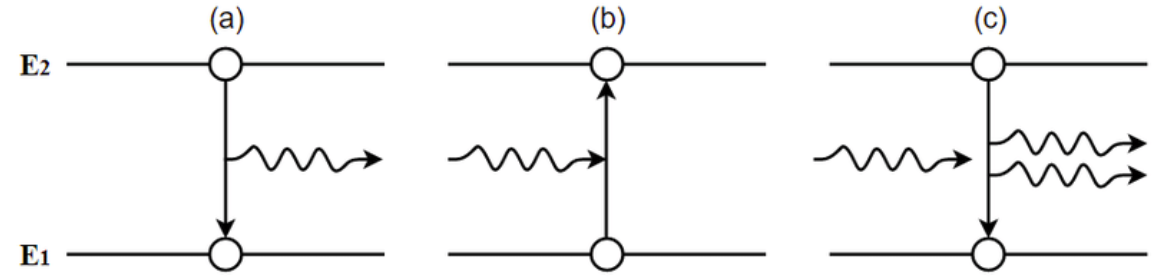
\includegraphics[width=\linewidth]{pictures/emission.png}
    \caption{Diagramtic representation of absorption (a), spontaneous emission (b) and stimulated emission (c) for a two state system.}
    \label{fig:emission}
\end{figure}

Different from the illustration in figure \ref{fig:emission} a laser needs a lasermedium
with more than two energy levels. In a two level system the Einsteincoefficients 
$B_{12}$ $B_{21}$ which describe the transition probability between the states are 
equal. Because of this the for the laser necessary population inversion is not possible
in a two level system. 

To achieve the population inversion a pump source has to impart energy into the system. 
In the case of a HeNe laser a electric discharger pumps energy into the pumpgas helium. 
The excited helium atoms collide with neon atoms, transfering their energy. The 
level schema is illustrated in figure \ref{fig:level}. 

\begin{figure}
    \centering
    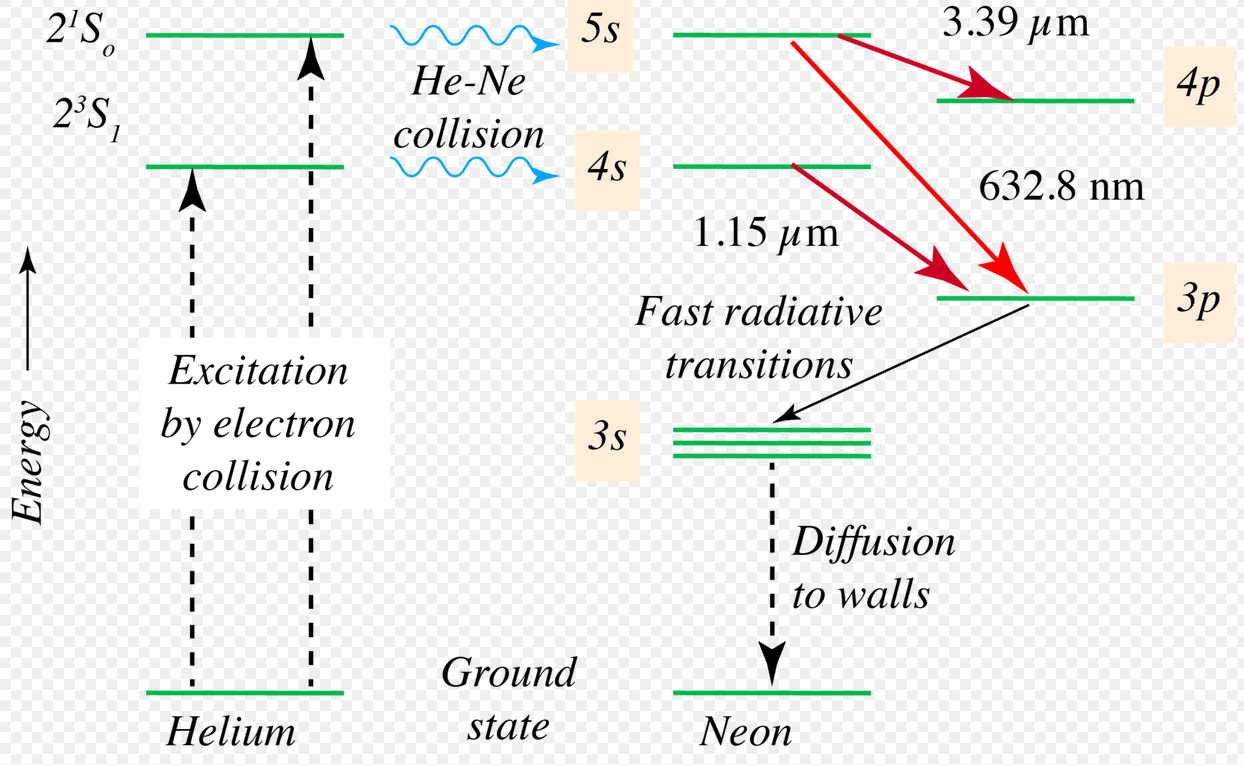
\includegraphics[width=\linewidth]{pictures/level.png}
    \caption{Diagramtic representation of the level schema if the HeNe lasers.}
    \label{fig:level}
\end{figure}
The transition from the 3s to the p2 state dominates the process resulting in the 
red laserlight with $\lambda = \SI{632.8}{\nano\meter}$.